\section{Background}

\begin{frame}\frametitle{Problema}

\large

\begin{itemize}[<+->]
\item
  Come è possibile \textbf{migliorare} ed \textbf{incentivare} la
  collaborazione nella produzione di software per la ricerca
  scientifica?
\item
  È possibile guardare all' Open Source come modello?
\end{itemize}

\end{frame}

\begin{frame}\frametitle{Incentivi \& Open Source}

\Large

\begin{itemize}[<+->]
\itemsep1pt\parskip0pt\parsep0pt
\item
  Early Literature

  \begin{itemize}[<+->]
  \itemsep1pt\parskip0pt\parsep0pt
  \item
    Idealismo e libertà di espressione
  \item
    Use-Value
  \item
    "\em{gift economy}"
  \end{itemize}
\item
  Recent Literature

  \begin{itemize}[<+->]
  \itemsep1pt\parskip0pt\parsep0pt
  \item
    Reputazione
  \item
    Possibilità di carriera
  \end{itemize}
\end{itemize}

\end{frame}

\begin{frame}\frametitle{Incentivi \& Software Scientifico}

\Large

\begin{itemize}[<+->]
\itemsep1pt\parskip0pt\parsep0pt
\item
  Mix di incentivi (reputazione)
\item
  \textbf{Domain shift}: software $\rightarrow$ scienza

  \begin{itemize}[<+->]
  \itemsep1pt\parskip0pt\parsep0pt
  \item
    discrepanze con altri contesti
  \item
    comportamenti palesemente controproducenti
  \end{itemize}
\end{itemize}

\end{frame}

\begin{frame}\frametitle{Collaborazione}

\begin{center}
\Large{Fasi della collaborazione}
\end{center}

\vspace{.5cm}

\begin{center}
    \includegraphics[width=\linewidth]{img/ciclo_collaborazione1}
\end{center}

\end{frame}

\section{Materiali \& Metodi}

\begin{frame}\frametitle{Cosa è BLAST (1)}

\Large

Il
\textbf{\alert{B}asic \alert{L}ocal \alert{A}lignment \alert{S}earch \alert{T}ool:}

\begin{itemize}[<+->]
\itemsep1pt\parskip0pt\parsep0pt
\item
  Creato nel 1990 e descritto in un articolo del \emph{Journal of
  Molecular Biology}
\item
  Concepito come un \textbf{algoritmo}
\item
  Divenuto poi un \textbf{tool software}
\item
  Attualmente sviluppato da un team del \emph{\textbf{National Center
  for Biotechnology Information}} (NCBI)
\end{itemize}

\end{frame}

\begin{frame}\frametitle{Cosa è BLAST (2)}

\Large{Funzionalità di BLAST:}

\begin{itemize}[<+->]
\itemsep1pt\parskip0pt\parsep0pt
\item
  Comparare fra loro sequenze biologiche primarie (ad es.
  \emph{aminoacidi})
\item
  Comparare fra loro sequenze di \emph{nucleotidi} del DNA
\item
  Comparare una sequenza in input con quelle provenienti da un database
  genomico
\item
  {[}\ldots{]}
\end{itemize}

\end{frame}

\begin{frame}\frametitle{Cosa è BLAST (3)}

\begin{center}
\Large{Sito ufficiale di NCBI BLAST}
\end{center}

\begin{center}
    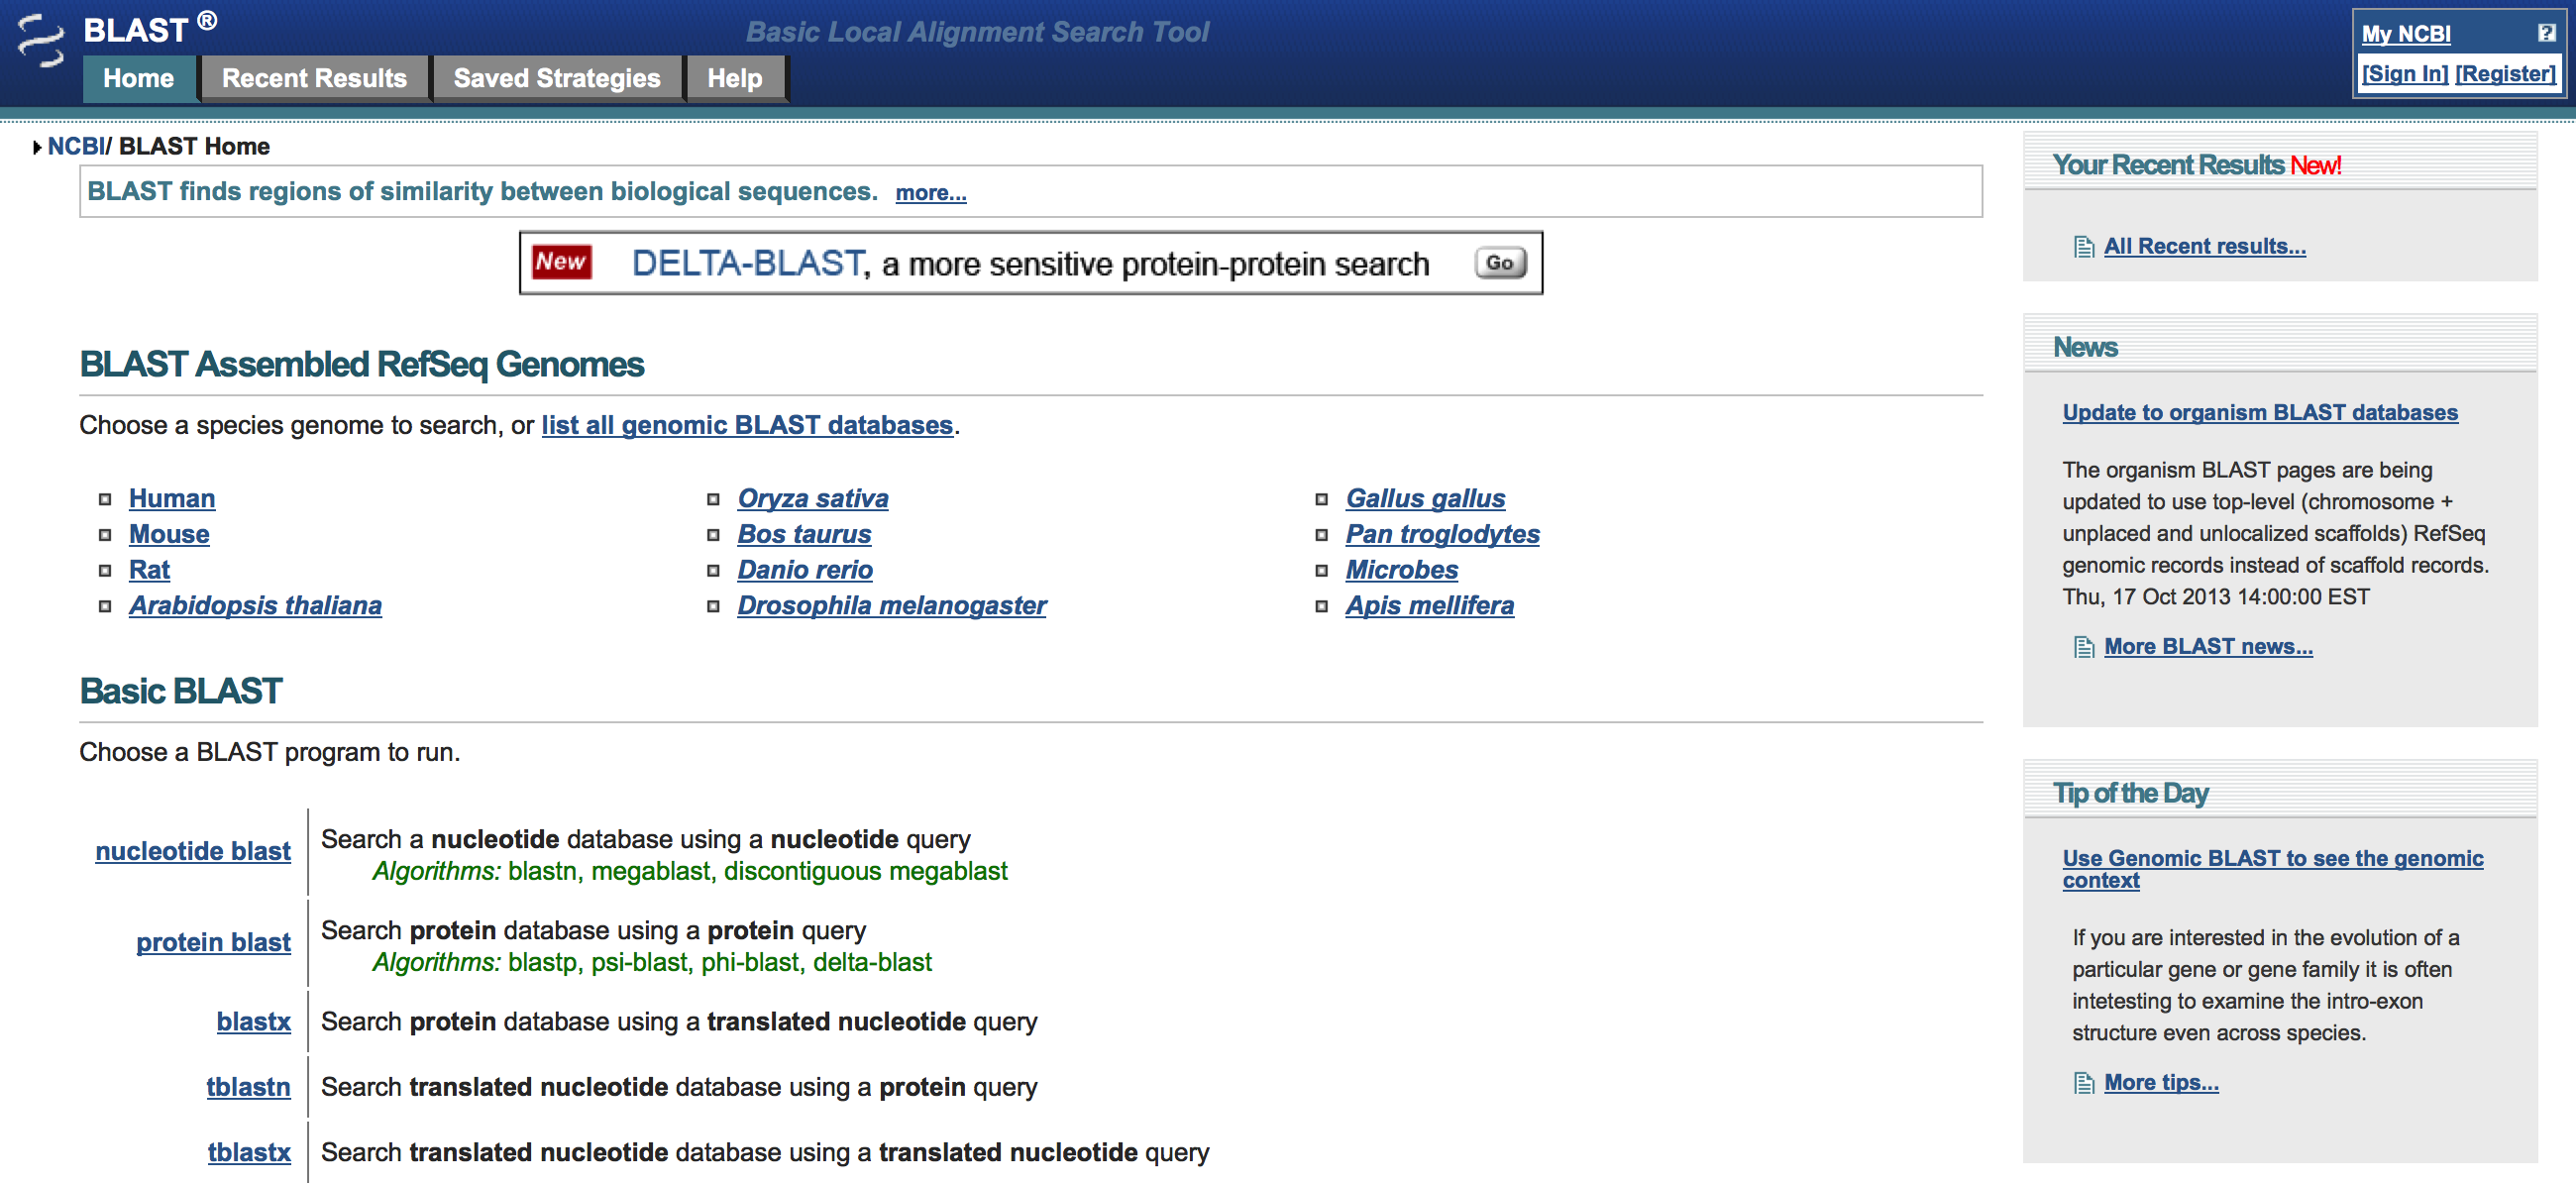
\includegraphics[scale=.12]{img/ncbi_blast}
\end{center}

\end{frame}

\begin{frame}\frametitle{Protocollo dello Studio}

\Large{Lo studio ha previsto:}

\begin{itemize}[<+->]
\itemsep1pt\parskip0pt\parsep0pt
\item
  Analisi dell'ecosistema \alert{\textbf{BLAST}}

  \begin{itemize}[<+->]
  \itemsep1pt\parskip0pt\parsep0pt
  \item
    Chi lo ha creato
  \item
    Chi ne cura manutenzione e sviluppo
  \item
    Quale codice è stato integrato
  \item
    Quali sono state le motivazioni
  \end{itemize}
\item
  Raccolta interviste semi-strutturate
\item
  Analisi qualitativa delle interviste
\item
  Ispezione della letteratura
\end{itemize}

\begin{alertblock}{Attenzione\dots}
Possibili bias dovuti alla ricerca nella letteratura
\end{alertblock}

\end{frame}

\begin{frame}\frametitle{Protocollo delle Interviste}

\Large

\begin{itemize}[<+->]
\itemsep1pt\parskip0pt\parsep0pt
\item
  Articolate in tre sezioni

  \begin{itemize}[<+->]
  \itemsep1pt\parskip0pt\parsep0pt
  \item
    Background dell'intervistato
  \item
    Natura del contributo/miglioramento a BLAST
  \item
    Motivazioni per il lavoro
  \end{itemize}
\item
  Interviste prevalentemente telefoniche
\item
  Interviste registrate
\end{itemize}

\end{frame}

\begin{frame}\frametitle{Materiale Raccolto}

\Large

\begin{itemize}[<+->]
\itemsep1pt\parskip0pt\parsep0pt
\item
  7 interviste con 8 intervistati
\item
  Rappresentativi delle 7 versioni di BLAST considerate
\item
  4 versioni individuate ma senza interviste

  \begin{itemize}[<+->]
  \itemsep1pt\parskip0pt\parsep0pt
  \item
    Letteratura
  \item
    Siti Web del progetto
  \end{itemize}
\end{itemize}

\end{frame}

\begin{frame}\frametitle{Analisi dei Dati}

\Large

\begin{itemize}[<+->]
\itemsep1pt\parskip0pt\parsep0pt
\item
  Sviluppo di transcript ed appunti
\item
  Ispezione della letteratura
\item
  Discussioni periodiche
\end{itemize}

\end{frame}

\begin{frame}\frametitle{Collaborazione \& Motivazioni}

\begin{center}
    \includegraphics[width=\linewidth]{img/ciclo_collaborazione2}
\end{center}

\end{frame}

\section{Risultati}

\begin{frame}\frametitle{Ecosistema BLAST}

\Large

\begin{itemize}[<+->]
\itemsep1pt\parskip0pt\parsep0pt
\item
  \alert{\textbf{NCBI BLAST}}
\item
  \alert{\textbf{BLAST+}}
\item
  \textbf{WU-BLAST} (ricerca di sequenze con gaps)
\item
  \textbf{Digital/Compaq BLAST} (ottimizzata per \emph{Alpha})
\item
  \textbf{Mac Os X Port}
\item
  \textbf{A/G BLAST} (versione ufficiale Apple)
\item
  \textbf{GPU BLAST} (sfrutta il parallelismo delle GPU Nvidia)
\item
  Altri (non inclusi nello studio)

  \begin{itemize}[<+->]
  \itemsep1pt\parskip0pt\parsep0pt
  \item
    Miglioramento di versione commerciale
  \item
    CUDA-BLAST
  \item
    FSA-BLAST
  \item
    CS-BLAST
  \end{itemize}
\end{itemize}

\end{frame}

\begin{frame}\frametitle{Analisi delle motivazioni (1)}

\Large{Motivazioni per lo \alert{sviluppo}:}

\begin{itemize}[<+->]
\itemsep1pt\parskip0pt\parsep0pt
\item
  Use-Value
\item
  Incremento dei profitti/vendita di Hardware
\item
  Divertimento
\item
  Reputazione accademica
\end{itemize}

\end{frame}

\begin{frame}\frametitle{Analisi delle motivazioni (2)}

\Large{Motivazioni per il \alert{rilascio}:}

\begin{itemize}[<+->]
\itemsep1pt\parskip0pt\parsep0pt
\item
  Etica
\item
  Accesso alle pubblicazioni
\item
  Incremento dei profitti
\end{itemize}

\end{frame}

\begin{frame}\frametitle{Analisi delle motivazioni (3)}

\Large{Motivazioni per l'\alert{integrazione}:}

\begin{itemize}[<+->]
\itemsep1pt\parskip0pt\parsep0pt
\item
  Riduzione dei costi di sviluppo/manutenzione
\item
  \alert{Contro-motivazione:} perdita della \emph{paternità} del
  contributo
\end{itemize}

\end{frame}

\begin{frame}\frametitle{Integrazione in BLAST}

\begin{figure}
\begin{center}
    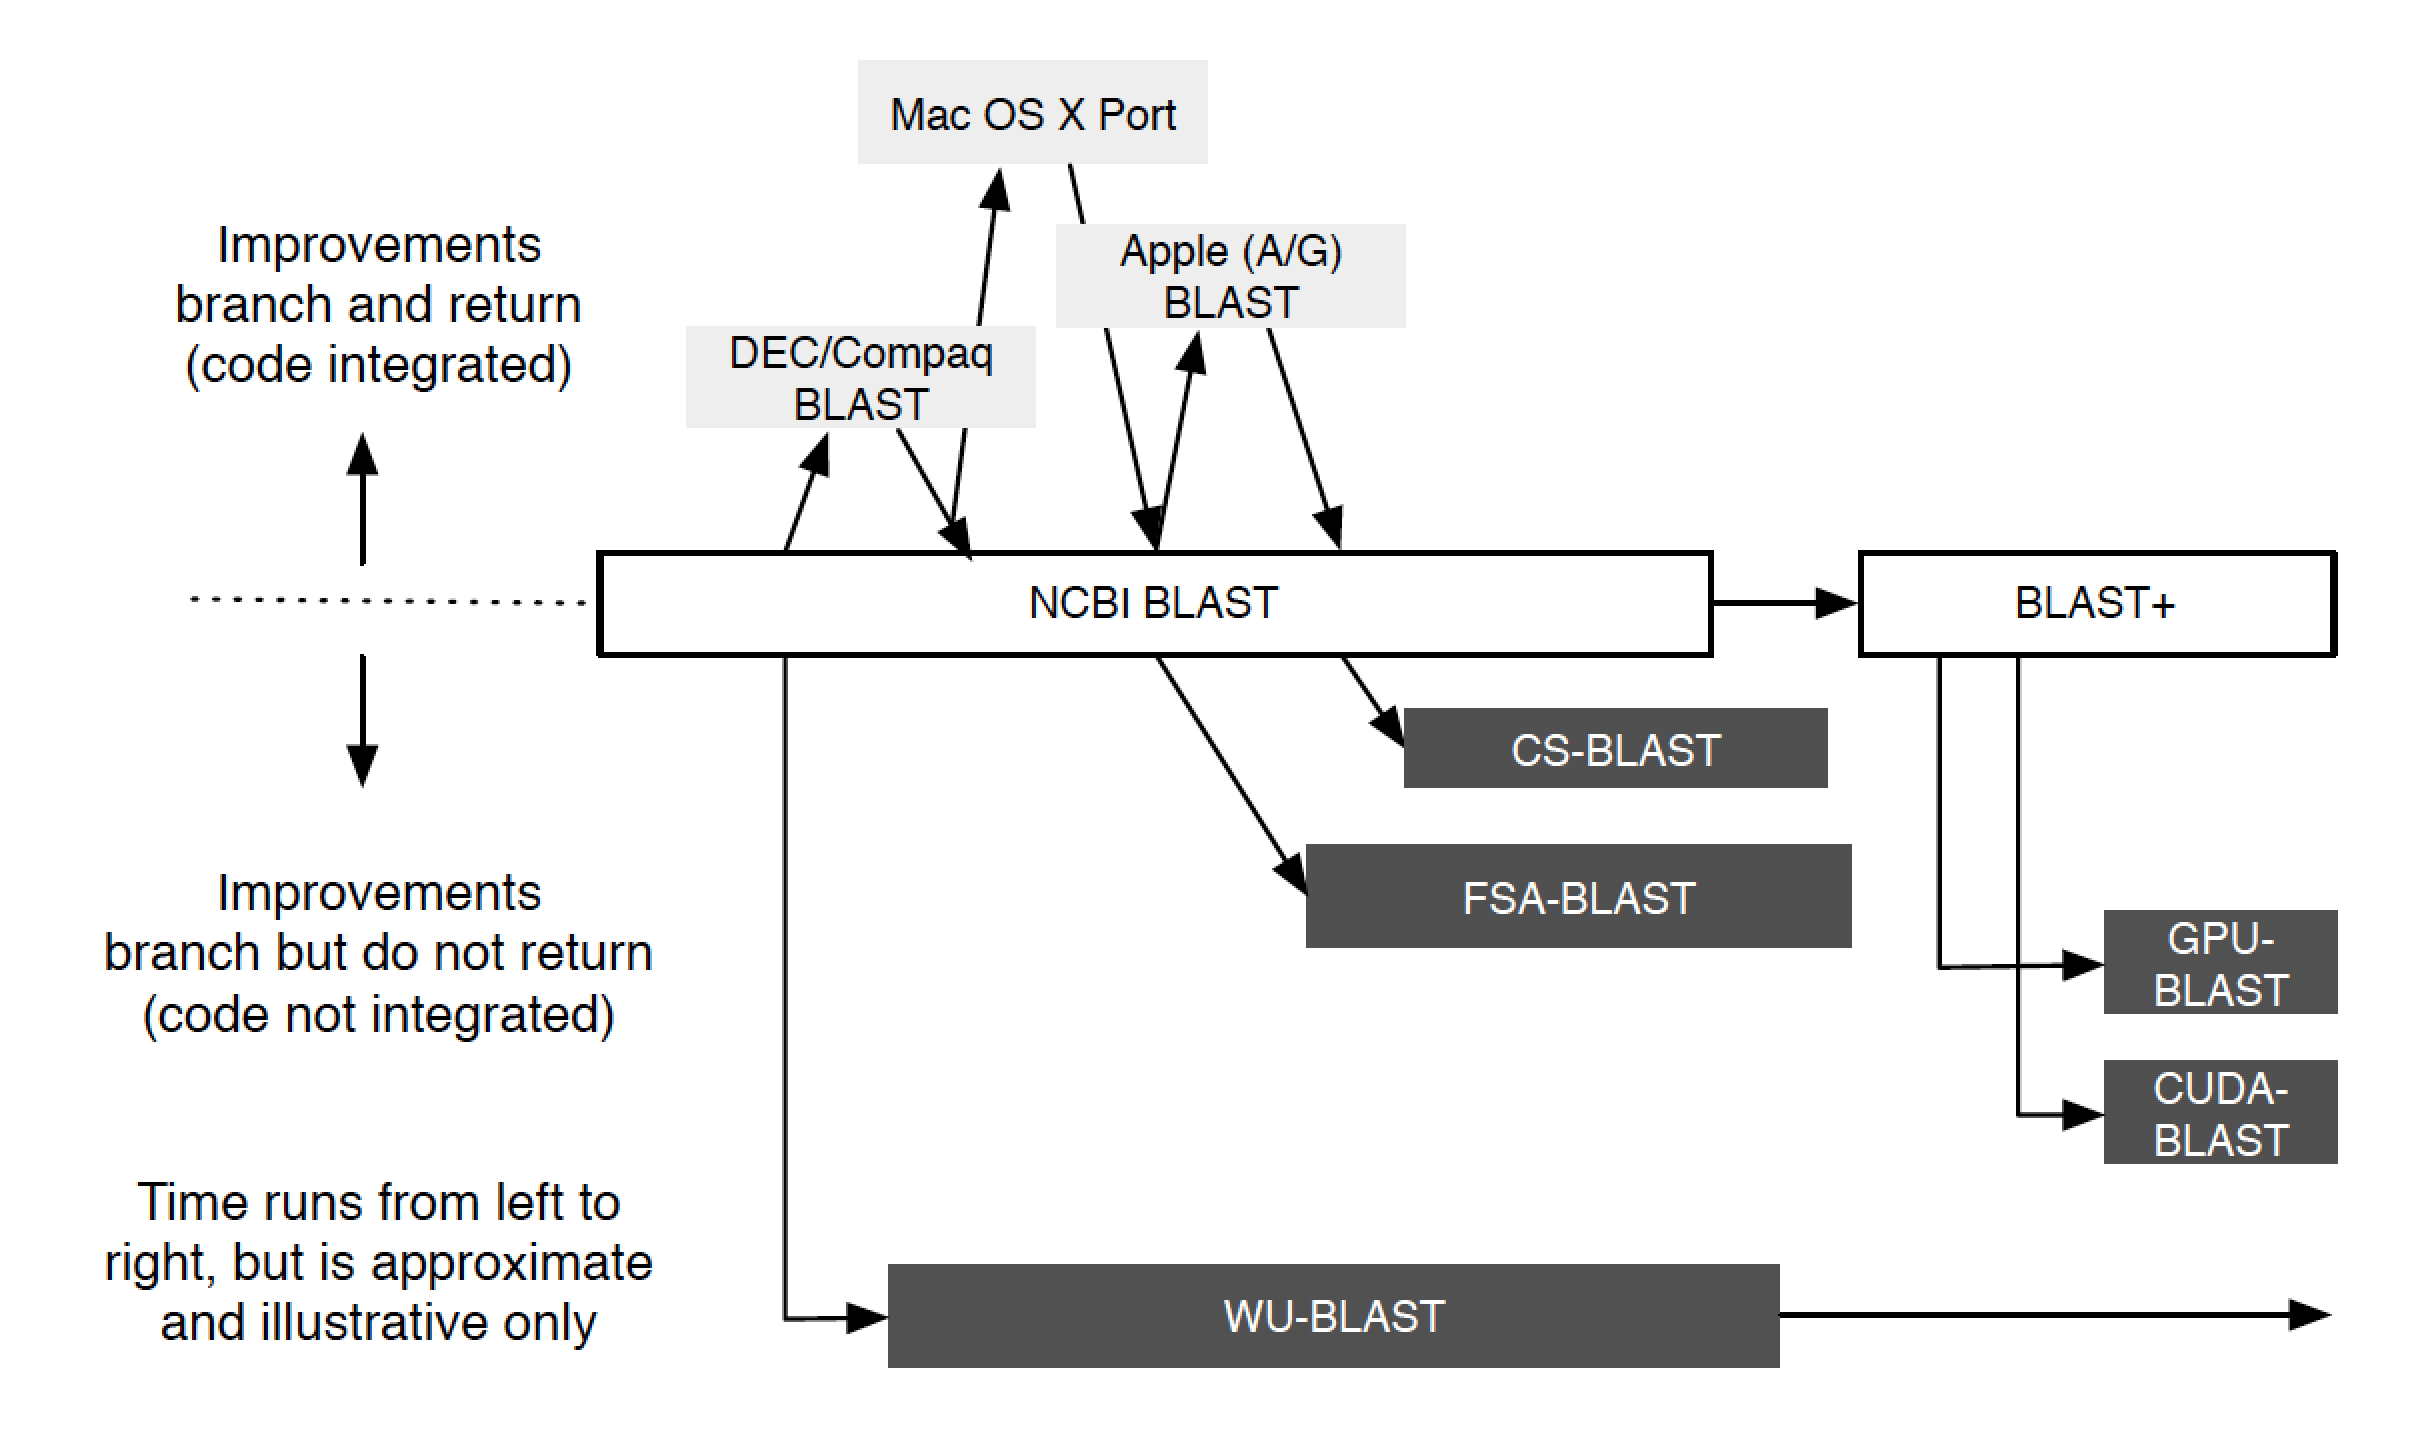
\includegraphics[scale=.25]{img/integration_blast}
\end{center}
\end{figure}

\textref{Fonte: Howison \& Herbsleb - "Incentives and Integration In Scientific Software Production", CSCW'13}

\end{frame}

\begin{frame}\frametitle{Quadro d'insieme}

\begin{center}
    \includegraphics[width=\textwidth]{img/incentives}
\end{center}

\end{frame}

\begin{frame}\frametitle{Possibili Spiegazioni}

\Large

\begin{enumerate}[<+->]
\def\labelenumi{\arabic{enumi}.}
\itemsep1pt\parskip0pt\parsep0pt
\item
  \textbf{Universalità del contributo}

  \begin{itemize}[<+->]
  \itemsep1pt\parskip0pt\parsep0pt
  \item
    \doublequoted{\em{Non è conveniente integrare contributi troppo specifici}}
  \item
    Non spiega la mancata integrazione di \emph{WU-BLAST} e \emph{GPU
    BLAST}
  \end{itemize}
\item
  \textbf{Costi di integrazione}

  \begin{itemize}[<+->]
  \itemsep1pt\parskip0pt\parsep0pt
  \item
    \doublequoted{\em{Il costo d'integrazione è minore in progetti modulari}}
  \item
    Sono stati integrati \emph{solo} contributi derivati da NCBI BLAST
  \end{itemize}
\item
  \textbf{Intenzioni degli autori}

  \begin{itemize}[<+->]
  \itemsep1pt\parskip0pt\parsep0pt
  \item
    \doublequoted{\em{L'integrazione (non)avviene su espressa volontà degli autori}}
  \item
    Spiegazione che si adatta al pattern osservato
  \end{itemize}
\end{enumerate}

\end{frame}

\begin{frame}\frametitle{Conflitto di Motivazioni}

\Large{La reputazione accademica come \alert{motivazione}:}

\begin{itemize}[<+->]
\itemsep1pt\parskip0pt\parsep0pt
\item
  Crea le condizioni per lo sviluppo e il rilascio di miglioramenti
\item
  \textbf{Non} per l'integrazione.
\item
  Per motivare l'integrazione sono richieste delle condizioni
  \alert{difficili} da soddisfare in un ottica di
  \alert{\em{mutuo beneficio}}
\end{itemize}

\end{frame}

\section{Discussione}

\begin{frame}\frametitle{Approccio alla discussione (1)}

\Large{\textbf{Due Domande:}}

\begin{enumerate}[<+->]
\def\labelenumi{\arabic{enumi}.}
\item
  Perché la reputazione sembra essere problematica nella produzione di
  software scientifico mentre altre motivazioni no?
\item
  Perché la reputazione costituisce un problema nella produzione di
  software scientifico mentre nel mondo Open Source no?
\end{enumerate}

\end{frame}

\begin{frame}\frametitle{Approccio alla discussione (2)}

\Large

\begin{itemize}[<+->]
\itemsep1pt\parskip0pt\parsep0pt
\item
  Analisi delle motivazioni osservate per

  \begin{itemize}[<+->]
  \itemsep1pt\parskip0pt\parsep0pt
  \item
    Sviluppo
  \item
    Rilascio
  \item
    Integrazione
  \end{itemize}
\item
  Punto di vista centrato sulla \alert{\em{divisione dei crediti}}
\end{itemize}

\begin{block}{Principio della divisione dei crediti:}

La collaborazione sarà tanto \alert{efficace} quanto più \alert{equa}
sarà la redistribuzione dei \emph{proventi} fra i partecipanti

\end{block}

\end{frame}

\begin{frame}\frametitle{Fun \& Learning}

\Large

\begin{itemize}[<+->]
\itemsep1pt\parskip0pt\parsep0pt
\item
  Immediatamente apprezzabile
\item
  Indipendente dalle performance del sistema
\item
  Indipendente dall'integrazione
\item
  Particolarmente adatta al mondo Open
\end{itemize}

\end{frame}

\begin{frame}\frametitle{Use-Value}

\Large

\begin{itemize}[<+->]
\itemsep1pt\parskip0pt\parsep0pt
\item
  Fenomeno ben noto nel Mondo Open Source
\item
  Presente anche nel Mondo Accademico e causa della produzione del c.d
  \emph{incidental software}
\item
  A volte \textbf{non} è un buon incentivo per il rilascio
\item
  Non è complementare all'integrazione
\end{itemize}

\end{frame}

\begin{frame}\frametitle{Denaro/profitti}

\Large

\begin{itemize}[<+->]
\itemsep1pt\parskip0pt\parsep0pt
\item
  Motivazione chiara
\item
  Facilita la divisione dei crediti
\end{itemize}

\end{frame}

\begin{frame}\frametitle{Reputazione}

\Large

\begin{itemize}[<+->]
\itemsep1pt\parskip0pt\parsep0pt
\item
  Potenzialmente problematica se vista in ottica di divisione dei
  crediti
\item
  Non si ottiene immediatamente nè indipendentemente
\item
  Non facilmente controllabile (in quanto attribuita da altri)
\item
  Suddivisione semplice se \alert{ogni} contributo individuale è
  \alert{chiaramente individuato} e riscontrabile nel prodotto finale
\end{itemize}

\end{frame}

\begin{frame}\frametitle{Reputazione:
\small{Open Source Vs Mondo Accademico}}

\Large{Meno problematica nel mondo Open Source rispetto al mondo accademico, per due ragioni:}

\begin{enumerate}[<+->]
\def\labelenumi{\arabic{enumi}.}
\itemsep1pt\parskip0pt\parsep0pt
\item
  Utilizzo di sistemi in grado di offrire un dettaglio dei contributi e
  dei relativi autori (as es. Github)
\item
  Meccanismo di ritorno in termini di crediti/reputazione più diretto
\end{enumerate}

\end{frame}

\begin{frame}\frametitle{Misura della Reputazione}

\Large{Il particolare sistema di reputazione accademica ha due implicazioni sulla produzione di Software Scientifico:}

\begin{enumerate}[<+->]
\def\labelenumi{\arabic{enumi}.}
\itemsep1pt\parskip0pt\parsep0pt
\item
  I contributi devono essere di una \emph{rilevanti} per essere
  \emph{degni} di pubblicazione
\item
  I contributi non hanno senso se non inclusi in pubblicazioni e/o
  citazioni i contributori figurano come autori
\end{enumerate}

\end{frame}

\section{Conclusioni}

\begin{frame}\frametitle{Conclusioni}

\Large

Quattro approcci per una possibile soluzione:

\begin{enumerate}[<+->]
\def\labelenumi{\arabic{enumi}.}
\itemsep1pt\parskip0pt\parsep0pt
\item
  Finanziare la fase di integrazione

  \begin{itemize}[<+->]
  \itemsep1pt\parskip0pt\parsep0pt
  \item
    in maniera \emph{diretta}
  \item
    attraverso la creazione di \doublequoted{facilitatori} (come ad es.
    \emph{Apache} e \emph{Debian})
  \end{itemize}
\item
  Cambio architetturale dei progetti di software scientifico
\item
  Cambio dell'\emph{economia} della reputazione accademica
\item
  Meccanismo di \emph{disaggregazione} a livello di pubblicazione dei
  contributi integrati
\end{enumerate}

\end{frame}
